\documentclass[
	paper=128mm:96mm,% like beamer
	fontsize=11pt,% like beamer
	pagesize ,% write page size to dvi or pdf
	parskip=half -,% paragraphs are separated by half a line
	numbers=noendperiod ,% no periods after section numbers
	captions=nooneline% same treatment of one/several lines
	,bibliography=totoc,listof=totoc, index=totoc,DIV=calc	
]{scrartcl}
\linespread {1.12}% enlarge line space
\usepackage[T1]{fontenc}                % Schriftenkodierung
\usepackage[latin1]{inputenc}       % Eingabekodierung Parameter
\usepackage[ngerman]{babel}    % mehrsprachiger Textsatz
\usepackage{fixltx2e}
\usepackage{ellipsis}
\usepackage[tracking=true]{microtype}
\usepackage{lmodern}                        % Ersatz fuer Computer Modern-Schriften
\usepackage{hfoldsty}
\usepackage{fourier}
\usepackage[osf,sc]{mathpazo}
\usepackage{xcolor}
\usepackage{calc}% working with lengths , counters etc.
\usepackage[includeheadfoot, top=3.5mm, bottom=3.5mm, left=5.5mm, right=5.5mm, headsep=6.5mm, footskip=8.5mm]{geometry}% set page layout parameters
\usepackage{scrpage2}% package for page style with not only uppercase letters in the head
\usepackage{titlesec}% for reducing space between ((sub)sub)sections and text
\usepackage{tocstyle}% for adjusting table of contents
\usepackage{mathtools}
%\usepackage{units}
%\usepackage{siunitx} % Benutzung: \SI{1}{\metre}
\usepackage{bm}
\usepackage{enumitem}
\usepackage{graphicx}
\usepackage{wrapfig}
%\renewcommand{\scriptsize}{\tiny}
%\usepackage[format=plain, labelformat=default, textformat=period, justification=centering, font=scriptsize, labelfont=bf]{caption}
%\captionsetup[figure]{name=Abb.}
%\captionsetup[wrapfigure]{name=Abb.}
%\captionsetup[wrapfigure]{margin=10pt}
\usepackage{tikz}
\usepackage{tabularx}
\usepackage{booktabs}
%\usepackage[numbers,square,comma,sort&compress,merge]{natbib}
\usepackage{url}
\usepackage[hidelinks%citebordercolor=white,linkbordercolor=white,urlbordercolor=white,
%,pdfpagemode=FullScreen%
]{hyperref}

\definecolor{mybgcolor}{HTML}{002F2F} %Colors: 002F2F, 046380, EFECCA, A7A37E, E6E2AF
\definecolor{mybgcolor2}{HTML}{EFECCA}
\definecolor{mydotcolor}{HTML}{046380}
\definecolor{mydotcolor2}{HTML}{A7A37E}
\definecolor{myfontcolor1}{HTML}{E6E2AF}
\definecolor{black}{rgb}{0,0,0}

\pagecolor{mybgcolor2}

\newcommand{\mycbox}[1]{\tikz{\path[draw=#1,fill=#1] (0,0) rectangle (4pt,4pt);}}

\newcommand{\mytitle}{Bericht des StAPF}
\newcommand{\myauthor}{StAPF}
\newcommand{\myuni}{St\"andiger Ausschuss der Physik-Fachschaften}
\newcommand{\mydate}{14. November 2013}

% page style
\pagestyle{scrheadings} % activates pagestyle from scrpage 2
\clearscrheadfoot % clear head and foot
\setkomafont{pageheadfoot}{\large\color{myfontcolor1}\sffamily}% setting for page head and foot
% optical vertical centering of page contents
\makeatletter
\renewcommand*{\@textbottom}{\vskip \z@ \@plus 1fil }
\newcommand*{\@texttop}{\vskip \z@ \@plus .5fil }
\addtolength{\parskip}{\z@ \@plus .25fil} % stretch parskip
\makeatother

\ihead{ % head left
	\hspace{-2mm}%
	\begin{tikzpicture}[remember picture, overlay]
	\node[xshift=\paperwidth/2, yshift=-\headheight] (mybar) at (current page.north west)[rectangle,fill,inner sep=0pt, minimum width=\paperwidth,minimum height=2\headheight, top color=mybgcolor!64, bottom color=mybgcolor]{}; % bar
	\node[below of=mybar,yshift=3.3mm, rectangle, shade,inner sep=0 pt, minimum width=128mm, minimum height=1.5mm, top color=black!50, bottom color=myfontcolor1]{}; %shadow
	\end{tikzpicture}%
	\Large{\textbf{\mytitle}}
}

\newlength{\footheight}
\setlength{\footheight}{8mm}
\addtokomafont{pagefoot}{\footnotesize} % size for foot
\setkomafont{pagenumber}{\color{myfontcolor1}} % white page number
\ifoot{% foot left
	\hspace{-2mm}%
	\begin{tikzpicture}[remember picture,overlay]
		\node[xshift=\paperwidth/2, yshift=\footheight/2] at (current page.south west)[rectangle, fill, inner sep=0pt, minimum width=\paperwidth, minimum height=\footheight, top color=mybgcolor!64, bottom color=mybgcolor]{}; % bar
	\end{tikzpicture}%
	\myauthor\ \raisebox{0.2mm}{$\bm{\vert}$}\ \myuni
}
\ofoot[\pagemark\hspace{-2mm}]{\pagemark\hspace{-2mm}}%foot right ( plain pages do also have page numbers )

\AtBeginDocument{\renewcaptionname{ngerman}{\contentsname}{Gliederung}}% change name of toc
\makeatletter
\newtocstyle[noonewithdot]{nodotnopagenumber}{% define tocstyle without dots and page numbers
	\settocfeature{pagenumberbox}{\@gobble}%
}
\makeatother
\usetocstyle{nodotnopagenumber}
%\setcounter{tocdepth}{2}
%\renewcommand*{\sectionmarkformat}{}
%\renewcommand*{\subsectionmarkformat}{}
\titlespacing*{\section}{-30pt}{0pt}{0pt}
%\titlespacing*{\subsection}{0pt}{0pt}{0pt}
%\titlespacing*{\subsubsection}{0pt}{0pt}{0pt}
%\titleformat{\section}{\color{white}\tiny}{}{0pt}{}
%\addtokomafont{subsubsection}{\large}
%\addtokomafont{subsection}{\Large}

%\automark[section]{\mytitle}

%\include{command}

\begin{document}
\thispagestyle{empty}
\begin{tikzpicture}[remember picture,overlay]
 \path [top color = mybgcolor!64,bottom color = mybgcolor] (current page.north east)rectangle (current page.south west);
\end{tikzpicture}
{\color{myfontcolor1}
	\begin{flushright}
%		\vspace{-0.5cm}
		{\Huge \textbf{\textsf{\mytitle}}}\\
		\vspace{.5cm}
		{\LARGE Winter-ZaPF 2013 in Wien}\\
		\vspace{.5cm}
		{\LARGE \mydate}
	\end{flushright}
}

\pagebreak
\addsec{Statistik} 
Anzahl teilnehmender Fachschaften an ZaPFen
 
\begin{figure}[hb]
	\begin{center}
		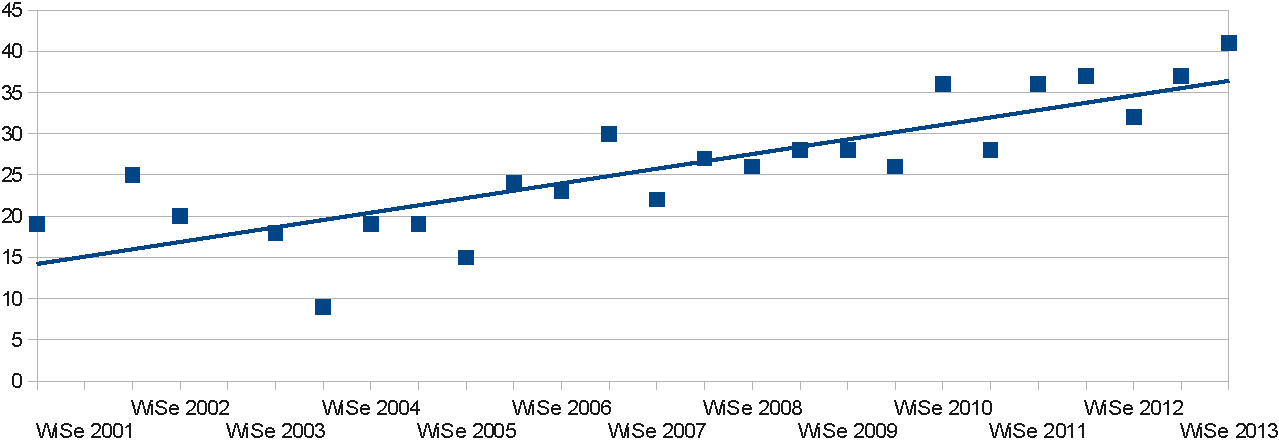
\includegraphics[width=.9\textwidth]{ZaPF-Teilnehmerliste_Statistik2013.pdf}
	\end{center}
\end{figure}
%\tableofcontents
\pagebreak
\addsec{Aktuelle Zusammensetzung}
	\begin{itemize}[label=\mycbox{mydotcolor}]
		\item \emph{Angelika Ambrusch (Uni Wien)}
		\item \emph{Benjamin Dummer (HU Berlin)}
		\item Bj"orn Guth (RWTH Aachen)
		\item Margret Heinze (LMU M"unchen)
		\item Tobias L"offler (Uni D"usseldorf)
	\end{itemize}
\pagebreak
\addsec{Versendung von Resolutionen etc.}
	\begin{itemize}[label=\mycbox{mydotcolor}]
		\item Problem bei Erstellung von Berichten und Resolutionen
		\begin{itemize}[label=\color{mydotcolor2}$\pmb\rightarrow$]
			\item Protokolle der Plenen:\quad \emph{zu sp"at \& zu ungenau}
		\end{itemize}
	\end{itemize}
\addsec{Studienf"uhrer}
	\begin{itemize}[label=\mycbox{mydotcolor}]
		\item Verantwortliche gesucht!
	\end{itemize}
\pagebreak
\addsec{Akkreditierungspool}
	\begin{itemize}[label=\mycbox{mydotcolor}]
		\item 17 Personen im Akkreditierungspool
		\begin{itemize}[label=\color{mydotcolor2}$\pmb\rightarrow$]
			\item Verl"angerung der Entsendung:\quad \emph{Julia Rietenbach (TU Dortmund) \& Eike Thesing (TU Kaiserlautern)}
		\end{itemize}
		\item 29. PVT in Dresden (21.06.-23.06.2013)
		\begin{itemize}[label=\color{mydotcolor2}$\pmb\rightarrow$]
			\item Beschwerdeausschuss: \quad \emph{Benjamin Dummer (HU Berlin)}
			\item Systemakkreditierungspool: \quad \emph{Margret Heinze (LMU M"unchen) \& Markus Gleich (FU Berlin)}
		\end{itemize}
		\item n"achstes PVT in Jena (29.11.-01.12.2013)
	\end{itemize}
\pagebreak
\addsec{Kontakt zu Fachschaften}
	\begin{itemize}[label=\mycbox{mydotcolor}]
		\item bislang ZaPF-inaktive Fachschaften eingeladen
		\begin{itemize}[label=\color{mydotcolor2}$\pmb\rightarrow$]
			\item einige hier in Wien
		\end{itemize}
		\item Berichte "uber aktuelle Situation und Geschehnisse angefragt
		\begin{itemize}[label=\color{mydotcolor2}$\pmb\rightarrow$]
			\item 9 Antworten bis jetzt...
			\item Online-Version:\quad  ZaPF-Wiki $\rightarrow$ Wien
		\end{itemize}
	\end{itemize}
\addsec{MeTaFa/Kontakt zu BuFaTas}
	\begin{itemize}[label=\mycbox{mydotcolor}]
		\item Online-Sitzung am 19.10.2013
		\begin{itemize}[label=\color{mydotcolor2}$\pmb\rightarrow$]
			\item Themen: \quad \emph{CHE, Erarbeitung zuk"unftiger Stellungnahmen \& Ver"offentlichungsplatform}
		\end{itemize}
		\item n"achstes physisches Treffen in Bamberg im M"arz \emph{(in Planung)}
		\item Besuche verschiedener BuFaTas: \quad \emph{Biologie, Soziologie, Philosophie, E-Technik}
	\end{itemize}

\pagebreak
\renewcommand{\mytitle}{Bericht des KommGrem}
\renewcommand{\myauthor}{KommGrem}
\renewcommand{\myuni}{Kommunikationsgremium \textit{zwischen jDPG und ZaPF}}
\addcontentsline{toc}{section}{Kommunikationsgremium}
\section*{Aktuelle Zusammensetzung}
	\begin{itemize}[label=\mycbox{mydotcolor}]
		\item ZaPF:\quad \emph{Margret Heinze (LMU M"unchen) \& \textbf{Benjamin Dummer (HU Berlin)}}
		\item jDPG: \quad \emph{Hejo Kerl (ETH Z"urich) \& Sebastian Heupts (Uni Heidelberg)}
	\end{itemize}
\section*{Sprecherschaft}
	\begin{itemize}[label=\mycbox{mydotcolor}]
		\item neue Sprecherin: \quad \emph{Margret Heinze (ZaPF)}
	\end{itemize}
\pagebreak
\section*{Besuche der KFP}
	\begin{itemize}[label=\mycbox{mydotcolor}]
		\item 21.-22.05.2013 in Bad Honnef \& 04.11.2013 in Berlin
	\end{itemize}
\section*{CHE-Hochschulranking}
	\begin{itemize}[label=\mycbox{mydotcolor}]
		\item Gemeinsame "`Task-Force"' von KFP, DPG, jDPG und ZaPF
	\end{itemize}
\section*{Bachelor-/Master-Umfrage}
	\begin{itemize}[label=\mycbox{mydotcolor}]
		\item Durchf"uhrung voraussichtlich SoSe 2014
	\end{itemize}
\pagebreak
\thispagestyle{empty}
\begin{tikzpicture}[remember picture,overlay]
 \path [top color = mybgcolor,bottom color = mybgcolor!64] (current page.north east)rectangle (current page.south west);
\end{tikzpicture}
{\color{myfontcolor1}
	\begin{center}
%		\vspace{-0.5cm}
		{\Huge \textbf{Fragen? Anregungen? ...}}\\
	\end{center}
}
\end{document}
